\section{Applications}
\label{sec:case}




% =======================================================================
\subsection{Testing for Trace Refinement}
 



% =======================================================================
\subsection{Testing for Failures Refinement}

For implementing the test case $U_F(p)$ with sub-processes $U_F(p,s)$, 
it is advisable to avoid an enumeration
of traces $s$ the reference process has run through. Instead, we calculate
the following auxiliary functions from $P$'s transition graph.
\begin{eqnarray*}
\text{initials} & : & N \fun \power (\Sigma) 
\\
\text{minHit} & : & N \fun \power\power(\Sigma)
\end{eqnarray*}
In a state $n = G(P)/s$, the set $\text{initials(n)}$ equals the events labelling
outgoing edges of $n$, so  $\text{initials(n)} = [P/s]^0$. Function $\text{minHit}$
maps $n$ to the set of all minimal hitting sets associated with the minimal acceptances
of $n$, so $\text{minHit}(n) = \text{minHit}(P/s)$. Then, using the transition function
of $t$ in addition to the two auxiliary functions, $U_F(p)$ can be re-written
as the failures-equivalent CSP process
\begin{eqnarray}
U_F^1(p) & = & U_F^1(p,0,\ii n)
\\
U_F^1(p,k,n) & = & \big( e:(\Sigma - \text{initials}(n)) \then \efail\then \Stop \big)
\label{eq:xufa}
\\ & & \extchoice \nonumber
\\ & & (\text{initials}(n) = \varnothing)    \&   \big( \epass \then \Stop \big)
\label{eq:xufb}
\\ & & \extchoice \nonumber
\\ & & (k < p) \& \big( e:\text{initials}(n) \then U_F^1(p,(k+1),t(n,e)) \big)
\label{eq:xufc}
\\ & & \extchoice \nonumber
\\ & & (k = p) \& \big( \sqcap_{H\in\text{minHit}(n)} ( e:H \then \epass \then\Stop   )  \big)
\label{eq:xufd}
\end{eqnarray}



% .....................................................................................
 \begin{figure}
 %%\hspace*{-40mm}
 \begin{center}
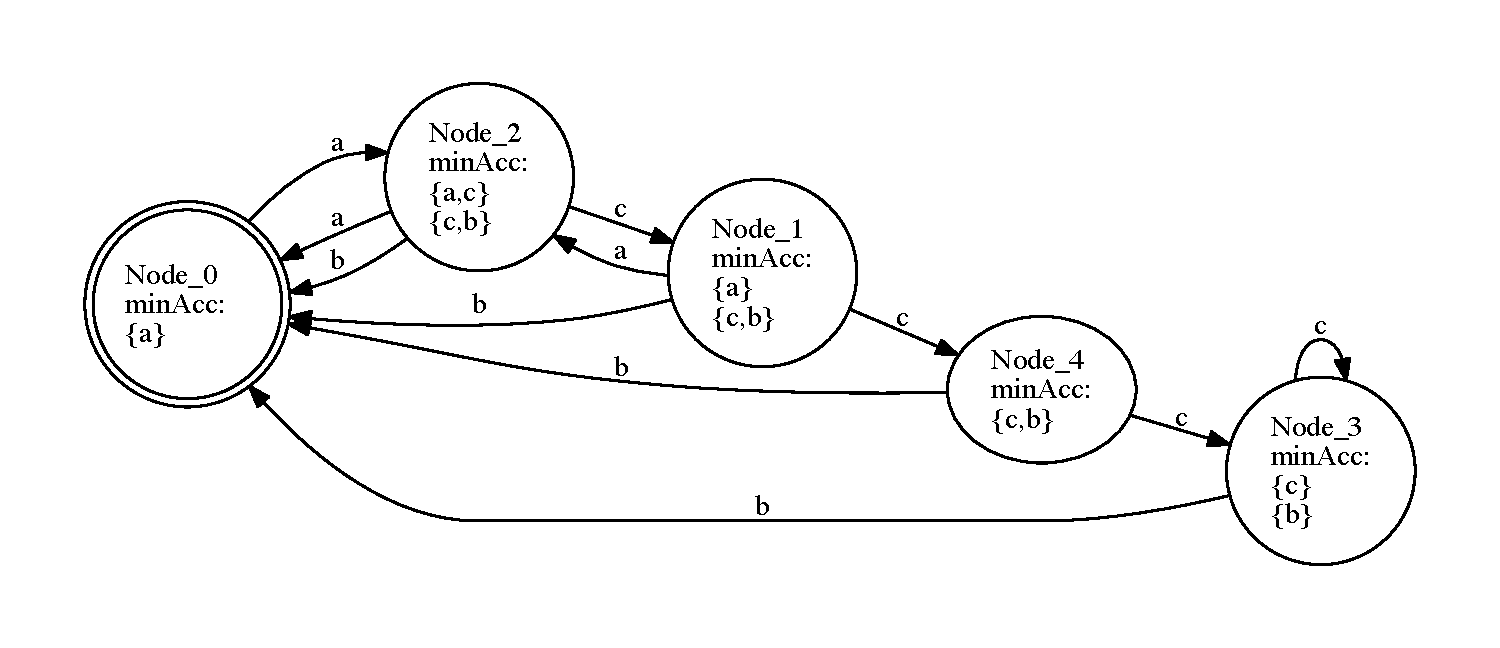
\includegraphics[width=\textwidth]{z_acc.pdf}
\end{center}
%%\vspace*{-10mm}
\caption{Normalised transition graph of faulty implementation $Z$  from Example~\ref{ex:uf1tests}.}
 \label{fig:tgZ}
 \end{figure}
% .......................................................................................



\begin{example}
\label{ex:uf1tests}
Consider the following erroneous implementation $Z$ of process $P$ from Example~\ref{ex:a}.
\begin{eqnarray*}
Z & = & a \then (Q_1 \intchoice R_1(r_{max},0))
\\
Q_1 & = & a\then Z \extchoice c\then Z
\\
R_1(r_{max},k) & = & (k < r_{max}) \& \big( c\then R_1(r_{max},k+1)\extchoice b\then Z  \big)
\\ & & \extchoice
\\ & & (k = r_{max}) \& \big( c\then R_1(r_{max},r_{max})\intchoice b\then Z  \big)
\end{eqnarray*}
It is easy to see (and can be checked with FDR4) that $Z$ is trace-equivalent to $P$. While $k < r_{max}$, process $Z$ also accepts the same sets of events as $P$. If, however,
sub-process $R_1(r_{max},k)$ runs through several recursions until condition 
$k = r_{max}$ is fulfilled, the process uses internal choice instead of external choice, and so this process state   no longer refines   the corresponding process state $R$ of the reference process $P$ in the failures model. For $r_{max} = 3$,   the
normalised transition graph of $Z$ is displayed in Fig.~\ref{fig:tgZ}.

Running the test $U_F^1(k)$ against $Z$ for $k=0,\dots,20$ ($G(P)$ has $p = 4$ states
and $G(Z)$ has $q=5$, so $pq=20$ is an upper bound for the test depth to be used 
according to Theorem~\ref{th:failurestest}), tests $U_F^1(0),\dots, U_F^1(3)$ are passed by $Z$, but $Z$ fails $U_F^1(4)$, because after  execution trace
\[
s = a.c.c.c, \qquad\text{(note that $G(Z)/s = \text{Node\_3}$ according to Fig.~\ref{fig:tgZ})},
\]
it may be the case that   $Z$  
only accepts $\{b\}$ due to internal choice and $U_F^1(4)$ 
-- also due to internal choice -- 
only accepts
the minimal hitting set $\{ c \}$ in union with the event $a\in (\Sigma - [P/s]^0)$. 
As
a consequence, $(Z\parallel[\Sigma] U_F^1(4))/s$ deadlocks for this execution, 
and the pass-event cannot be
produced. Another failing execution would be the situation where $Z/s$ choses to
accept only $\{c \}$, while $U_F^1(4))/s$ choses to accept only $\{a,b\}$.

Therefore, 
\[
(\epass\then \Stop)\not\lessdet_F  (Z\parallel[\Sigma] U_F^1(4)),
\]
and the test fails.
\xbox
\end{example}
 
 


% ====================================================================== 